% Supplementary Information for:
% "Decoding Real-Space Neural Wavefunctions for Post-Hartree-Fock Quantum Chemistry"
%
% Compile: pdflatex supp && bibtex supp && pdflatex supp && pdflatex supp
\documentclass[journal=jctcce,manuscript=suppinfo,layout=traditional]{achemso}

\usepackage{amsmath,amssymb,bm,booktabs,graphicx,xcolor,hyperref,siunitx}
\usepackage[version=4]{mhchem}
\usepackage{algorithm}
\usepackage{algpseudocode}

\author{Tae In Kim}
\altaffiliation{Contributed equally.}
\affiliation{Department of Energy Science, Sungkyunkwan University, Suwon 16419, Korea}
\author{Tae Hyeon Park}
\altaffiliation{Contributed equally.}
\affiliation{Department of Energy Science, Sungkyunkwan University, Suwon 16419, Korea}
\author{Gi Beom Sim}
\altaffiliation{Contributed equally.}
\affiliation{Department of Energy Science, Sungkyunkwan University, Suwon 16419, Korea}
\author{Yanmei Zang}
\affiliation{Department of Energy Science, Sungkyunkwan University, Suwon 16419, Korea}
\author{Xiaorong Zou}
\affiliation{Center for 2D Quantum Heterostructures, Institute for Basic Science, Suwon 16419, Korea}
\author{Libor Veis}
\email{libor.veis@jh-inst.cas.cz}
\affiliation{J. Heyrovsky Institute of Physical Chemistry, Czech Academy of Sciences, Prague 18223, Czechia}
\author{Soohaeng Yoo Willow}
\email{sy7willow@skku.edu}
\affiliation{Department of Energy Science, Sungkyunkwan University, Suwon 16419, Korea}
\author{D. ChangMo Yang}
\email{dcyang@skku.edu}
\affiliation{Department of Energy Science, Sungkyunkwan University, Suwon 16419, Korea}
\author{Chang Woo Myung}
\email{cwmyung@skku.edu}
\affiliation{Center for 2D Quantum Heterostructures, Institute for Basic Science, Suwon 16419, Korea}
\affiliation{Department of Energy Science, Sungkyunkwan University, Suwon 16419, Korea}

\title{Supplementary Information for: Decoding Real-Space Neural
       Wavefunctions for Post-Hartree--Fock Quantum Chemistry}

\begin{document}

\renewcommand{\thesection}{S\arabic{section}}
\renewcommand{\thefigure}{S\arabic{figure}}
\renewcommand{\thetable}{S\arabic{table}}
\renewcommand{\theequation}{S\arabic{equation}}
\setcounter{section}{0}
\setcounter{figure}{0}
\setcounter{table}{0}
\setcounter{equation}{0}

\section*{Contents}
\begin{itemize}
\item S1. Implementation details
\item S2. Ground-state recovery extras: symmetry diagnostics and NN-NO bootstrap
\item S3. Converged-NN validation on \ce{BeH2}/cc-pVDZ
\item S4. Selected-CI warm-start with $\widehat c$
\item S5. NES-VMC excited states: full pipeline
\item S6. Reduced density matrices and chemical interpretation
\item S7. Failure modes and explicit deferrals (\ce{C2}, \ce{H8} NEVPT2, \ce{Cr2})
\end{itemize}

%==========================================================================
% S1: Implementation details (moved from main §IV)
%==========================================================================
\section{Implementation details}
\label{sec:supp_implementation}

The complete framework, from a trained NN-VMC checkpoint to a
chemist-readable CI vector and downstream observables, is summarised
in Algorithm~\ref{alg:framework}.

\begin{algorithm}[h]
\caption{NN-VMC $\to$ chemist-language CI vector via the
\textsc{OmegaQMC.cs} framework. The only mean-field input is one
RHF SCF cycle; no CASSCF, CASCI, or FCI is invoked. All
downstream observables (NTOs, NEVPT2, 1-/2-RDM properties) follow
from the returned $\widehat c^{\rm NN-NO,\, Lasso}$ and
$C_{\rm NN-NO}$.}
\label{alg:framework}
\begin{algorithmic}[1]
\Require Trained trial $\Psi_{\rm NN}$, walker bank
         $\{R_k\}_{k=1}^{K_s} \sim |\Psi_{\rm NN}|^2/Z$,
         AO basis $\{\chi_\mu\}$, chemist vocabulary
         $\mathrm{CAS}(n_{\rm cas},(n_\alpha^{\rm cas},n_\beta^{\rm cas}))$,
         threshold $\lambda$
\State $C_{\rm HF} \gets \textsc{RHF}(\mathrm{mol})$
       \Comment{one SCF cycle, $\sim$ seconds}
\State Enumerate candidate set $\mathcal{S} \gets
       \{ (\mathrm{occ}^\alpha,\mathrm{occ}^\beta) :
          \mathrm{occ}^\sigma \subset \{0,\dots,n_{\rm cas}-1\},
          |\mathrm{occ}^\sigma| = n_\sigma^{\rm cas} \}$
       \Comment{$|\mathcal{S}| = \binom{n_{\rm cas}}{n_\alpha^{\rm cas}}
                                  \binom{n_{\rm cas}}{n_\beta^{\rm cas}}$}
\State $v^{\rm HF}_p(\mathbf{r}_i^k) \gets
       \sum_\mu C_{\rm HF}[\mu,p]\,\chi_\mu(\mathbf{r}_i^k)$
       \Comment{Pass 1: orbital values, $K_s$ walker positions}
\For{each $I \in \mathcal{S}$}
  \State $\widetilde c_I^{\,\rm HF} \gets
         \frac{1}{K_s}\sum_{k=1}^{K_s}
         \frac{D_I^{\rm HF}(R_k)}{\Psi_{\rm NN}(R_k)}$
         \Comment{sample-mean overlap estimator}
\EndFor
\State $\widehat c^{\rm HF} \gets
       \widetilde c^{\,\rm HF} \,/\, \|\widetilde c^{\,\rm HF}\|_2$
       \Comment{$L_2$ normalisation absorbs $\sqrt{Z}$}
\State $\widehat \gamma^{\rm HF}_{pq} \gets
       \sum_{I,J \in \mathcal{S}}
       \widehat c^{\rm HF}_I \, \widehat c^{\rm HF}_J \,
       \langle D_I | a_p^\dagger a_q | D_J \rangle$
       \Comment{PySCF \texttt{make\_rdm1}}
\State $\widehat \gamma^{\rm HF} \gets
       \tfrac{1}{2}(\widehat \gamma^{\rm HF} +
                    \widehat \gamma^{\rm HF\,\top})$
       \Comment{symmetrise}
\State $(n_p^{\rm NN}, U) \gets
       \textsc{Eigh}(\widehat \gamma^{\rm HF})$
       \Comment{NN-NOs = columns of $U$ in HF coordinates}
\State $C_{\rm NN-NO} \gets C_{\rm HF}\,U$
       \Comment{Pass 2 orbital coefficients in AO basis}
\State $v^{\rm NN-NO}_p(\mathbf{r}_i^k) \gets
       \sum_\mu C_{\rm NN-NO}[\mu,p]\,\chi_\mu(\mathbf{r}_i^k)$
       \Comment{Pass 2: re-evaluate orbitals on the same walker bank}
\For{each $I \in \mathcal{S}$}
  \State $\widetilde c_I^{\,\rm NN-NO} \gets
         \frac{1}{K_s}\sum_{k=1}^{K_s}
         \frac{D_I^{\rm NN-NO}(R_k)}{\Psi_{\rm NN}(R_k)}$
\EndFor
\State $\widehat c^{\rm NN-NO} \gets
       \widetilde c^{\,\rm NN-NO} \,/\,
       \|\widetilde c^{\,\rm NN-NO}\|_2$
\State $\widehat c^{\rm NN-NO,\,\rm Lasso}_I \gets
       \mathrm{soft}_\lambda(\widehat c^{\rm NN-NO}_I)
       = \mathrm{sign}(\widehat c^{\rm NN-NO}_I)
         \max(|\widehat c^{\rm NN-NO}_I| - \lambda, 0)$
       \Comment{soft-thresholding (main-text \S III.D);
                reference determinant excluded}
\State \Return $\widehat c^{\rm NN-NO,\,\rm Lasso}$ and
       $C_{\rm NN-NO}$ for downstream NTOs / NEVPT2 / RDM analysis
\end{algorithmic}
\end{algorithm}

\subsection{Natural-orbital basis}
\label{sec:nn_no_source}

In the implementation we adopt the natural-orbital (NO) basis
$\{\eta_p\}$ defined as the eigenvectors of the one-particle reduced
density matrix
$\gamma_{pq} = \langle \widetilde{\Psi} | a_p^{\dagger} a_q
| \widetilde{\Psi} \rangle$. The natural-orbital ansatz traces back to
L\"owdin~\cite{Lowdin1955natural}; in QMC practice it has been used
since the early 2000s as the sparsifying frame for selected-CI and
subsequent
processing~\cite{Per2008NOVMC,Filippi2000NO,Bytautas2013NOs}. Two
NO sources are admissible:
(i) the NOs of $\widetilde{\Psi}_{\mathrm{NN}}$ itself, computed from
the Monte Carlo estimator
$\widehat{\gamma}_{pq} = \langle \chi_p^{\dagger} \chi_q
\rangle_{|\Psi_{\mathrm{NN}}|^2}$;
(ii) the NOs of the FCI eigenstate $\Psi_{\mathrm{FCI}}(B)$ in the
chosen Gaussian basis $B$, computed once via PySCF~\cite{PySCF2020}.
The two coincide in the limit
$\widetilde{\Psi}_{\mathrm{NN}} \to \widetilde{\Psi}_{\mathrm{FCI}}(B)$.
We use (ii) throughout this work because it provides a fixed external
reference frame in which the head-to-head comparison
$\widehat{c} \leftrightarrow c^{\mathrm{FCI}}$ is unambiguous, and
because (i) carries the additional Monte Carlo variance of the 1-RDM
estimator on top of the f-vector variance. For a NN trial wavefunction
substantially below the FCI(B) energy --- as occurs when the NN
captures correlation beyond the basis $B$ --- (ii) introduces a
basis-misalignment bias that we quantify in
main-text \S V.B.

\subsection{Walker bank and signed-$\Psi$ evaluation}

The NN-VMC driver in our implementation
(\textsc{OmegaQMC}~\cite{Pfau2020FermiNet,Hermann2020PauliNet})
supports a \texttt{dump\_walkers\_path} argument that streams the
post-block walker configurations and $\log|\Psi_{\mathrm{NN}}|$ to an
HDF5 file. Concurrent VMC energy evaluation and walker dump add
negligible overhead because each production block is already a
synchronous JAX scan~\cite{JAX2018}.

To evaluate $f_I$ we require the signed
$\Psi_{\mathrm{NN}}(\mathbf{R})$, not just the magnitude. The model
output object in OmegaQMC carries both $\mathrm{sign}(\Psi)$ and
$\log|\Psi|$; we expose a \texttt{log\_psi.signed} attribute on the
adapter callable returning $(\mathrm{sign}, \log|\Psi|)$ that the CS
pipeline batches via \texttt{jax.vmap}~\cite{JAX2018,Heek2024Flax} over
the loaded walker bank. The orbital evaluations
$\eta_p(\mathbf{r}_i^{\sigma})$ are computed once via a PySCF
\texttt{eval\_gto} call on the flattened bank.

\subsection{Streaming evaluation and chunking}

The full $f_I$ matrix has dimensions $(N_{\mathrm{det}},
K_s^{\mathrm{max}})$ which can exceed available memory for
production-scale runs ($N_{\mathrm{det}} \sim 10^6$,
$K_s^{\mathrm{max}} \sim 10^5$). We stream the evaluation in
determinant chunks of size $L$: for each chunk, evaluate $f_I$ for the
$L$ determinants across the full walker bank, accumulate the chunk
contribution to the per-$(K_s, \text{seed})$ sample means, and
discard. Memory is bounded by $L \cdot K_s^{\mathrm{max}}$ regardless
of $N_{\mathrm{det}}$. Chunked and full-matrix evaluation are
bit-identical (verified as a unit test in the released code).

\subsection{Spin-layout convention}

A subtle but practically important point concerns the layout of
electrons within the walker array. NN-VMC architectures based on
spin-resolved equivariant networks adopt the
\emph{interleaved} convention in which spin-up electrons occupy
even-indexed positions and spin-down odd-indexed positions
(e.g.\ FermiNet~\cite{Pfau2020FermiNet},
PsiFormer~\cite{vonGlehn2023PsiFormer},
PauliNet~\cite{Hermann2020PauliNet}). The PySCF CI convention is the
\emph{grouped} layout with all spin-up first followed by spin-down,
matching the standard block-diagonal Slater determinant form. For
$N_{\alpha} = N_{\beta} = 1$ the two coincide, but for
$N_{\sigma} \ge 2$ the spin-row assignment in the Slater determinant
$D_I$ (main-text Eq.~3) must be performed in a single consistent convention.
Our implementation receives walkers in the interleaved convention and
permutes to grouped before the determinant evaluation. The released
code includes unit tests verifying that mis-specifying the convention
produces a recovery error at least an order of magnitude larger than
the correct convention, and that recovery quality is invariant to the
overall scale of the trial wavefunction.

%==========================================================================
% S2: Ground-state recovery extras
%==========================================================================
\section{Ground-state recovery: symmetry diagnostics and NN-NO bootstrap}
\label{sec:supp_groundstate}

\subsection{Symmetry diagnostics}
\label{sec:supp_symmetry_diag}

For a singlet ground state, the spatial wavefunction is symmetric
under $\alpha \leftrightarrow \beta$ permutation, requiring
$c_{(\mathrm{occ}^{\alpha}, \mathrm{occ}^{\beta})}
= c_{(\mathrm{occ}^{\beta}, \mathrm{occ}^{\alpha})}$ when the alpha and
beta strings differ. PySCF FCI enforces this exactly; the recovered
$\widehat{c}$ from a separate-$\alpha\beta$ architecture
(PsiFormer~\cite{vonGlehn2023PsiFormer},
FermiNet~\cite{Pfau2020FermiNet}) shows residual asymmetry of order
$1\%$--$3\%$, e.g.\ $\widehat{c}_{((1,2),(0,3))} - \widehat{c}_{((0,3),(1,2))}
= -0.011$ for the H4 linear case. This is a direct probe of spatial
symmetry breaking in the trained NN, surfaced by the recovery
pipeline and not visible from the VMC energy alone.

\paragraph{Quantitative spin-contamination diagnostic.}
The spin contamination of the recovered $\widehat c$ is computable
via the standard CI-vector contraction
$\langle S^2\rangle = \sum_{IJ} \widehat c_I \widehat c_J
\langle D_I | \hat S^2 | D_J\rangle$ (\texttt{pyscf.fci.spin\_op.spin\_square0}).
On the converged \ce{BeH2}/cc-pVDZ cell (5000 SR iters,
\S\ref{sec:supp_beh2}) the recovered
$\langle S^2\rangle^{\widehat c} = 0.137$ vs the FCI value
$\langle S^2\rangle^{\rm FCI} \approx 0$; on \ce{H4}/cc-pVDZ
the recovered value is $0.096$ vs FCI $\approx 0$. Both are
small-but-finite deviations from the singlet target, quantifying the
$\alpha$--$\beta$ asymmetry that the FermiNet separate-spin path
architecture introduces. The corresponding spin multiplicities
($1.24$ for \ce{BeH2} and $1.18$ for \ce{H4}, vs the singlet target
$1.00$) translate the contamination into the familiar chemist's-
language unit. These numbers are reproducible via
\texttt{examples/run\_cs\_s2\_2rdm.py}; JSON outputs in
\texttt{data/beh2\_s2\_2rdm.json} and \texttt{data/h4\_s2\_2rdm.json}.

\subsection{Self-consistent NN-NO frame (CASSCF/CASCI-free deployment)}
\label{sec:nn_no_self_consistent}

The Source-2 path of \S\ref{sec:nn_no_source} relies on a one-time
CASCI calculation to supply the natural-orbital frame and the candidate
determinant set. That CI-level dependency can be removed by deriving
the natural orbitals from the NN-VMC 1-RDM itself and supplying the
candidate set as a vocabulary-choice combinatorial object. The
framework as deployed requires exactly one mean-field input:
a single Hartree--Fock (RHF) SCF cycle to anchor the Pass-1 orbital
frame, costing seconds for any first- or second-row system and
introducing no CASSCF, CASCI, or FCI machinery. The Pass-1 c-vector
in the HF frame is then used to build the trial 1-RDM, whose
eigenvectors are the NN-NOs; Pass 2 in NN-NO basis yields the
self-consistent CI vector.

Three candidate-set strategies are admissible (CAS index structure on
the top-occupation NN-NOs; HF-rank cutoff with all $S{+}D$ excitations;
NN-guided selected-CI sweep). The CAS-index strategy is the cleanest
in math and the most robust in practice because the only failure mode
--- vocabulary too small --- is directly diagnosed by the
match-overlap statistic of main-text \S VI / SI \S\ref{sec:supp_excited}, with no
Monte-Carlo-noise-driven Type~I/II support-recovery error budget to
tune. We deploy it here on the same \ce{H2}/cc-pVDZ cell as
main-text \S V.A, choosing the full $(n_\alpha{=}1, n_\beta{=}1)$
candidate enumeration in the 10-AO basis (100 determinants, no CAS
truncation needed for two electrons).

The bootstrap is a two-pass workflow.
\emph{Pass~1:} Hartree--Fock orbitals from a one-shot RHF call (no
FCI, no CASCI); run the standard CS pipeline of main-text \S III
to produce $\widehat c^{\rm HF}$; construct the 1-RDM
$\widehat \gamma^{\rm HF}_{pq} = \langle \widehat c^{\rm HF} |
a_p^\dagger a_q | \widehat c^{\rm HF} \rangle$ via PySCF's
\texttt{make\_rdm1}; symmetrise and diagonalise to obtain the NN-NO
rotation $U$ and the NN-NO occupations $\{n_p^{\rm NN}\}$.
\emph{Pass~2:} transform the AO-basis NO coefficients
$\eta^{\rm NN-NO}_{p, {\rm AO}} = (\text{mo}_{\rm hf})_{,U} U_{,p}$ and
re-run the CS pipeline to obtain $\widehat c^{\rm NN-NO}$ in the
self-consistent frame. The walker bank is unchanged across passes;
only \texttt{evaluate\_orbitals\_on\_walkers} is re-evaluated.
Total wall time on the H2 cell: 14\,seconds on a single
RTX 4090.

Table~\ref{tab:h2_nn_no} reports the result against the FCI-NO
calibration of main-text \S V.A. The HF coefficient recovery in the
self-consistent NN-NO frame ($\widehat c_{((0)(0))} = +0.97035$)
matches the FCI value ($+0.97023$) to $0.01\%$, slightly tighter than
the $0.05\%$ recovery in the FCI-NO frame. The NN-NO occupations
$\{1.8914, 0.0905, 0.0057, 0.0045\}$ agree with FCI-NO occupations
$\{1.8827, 0.1107, 0.0037, 0.0010\}$ to within the expected
NN-vs-FCI residual ($\sim 1$~m$E_{\rm h}$ in this cell), with the
small NN-vs-FCI shift on the LUMO occupation $0.0905$ vs $0.1107$
reflecting the same correlation balance that produces the $1.2$~m$E_{\rm
h}$ NN-FCI energy gap. The frame alignment between NN-NOs and
FCI-NOs --- measured as the diagonal of $|U^\dagger S V|$ where $U$
and $V$ are the two NO sets in the AO frame and $S$ is the AO overlap
matrix --- is $0.9997$ on the dominant $\sigma_g$ orbital and
$0.9950$ on the LUMO $\sigma_u^*$; the deeper orbitals are
near-degenerate pairs that rotate freely without affecting the
recovered $\widehat c$. The reproducibility script is
\texttt{examples/run\_h2\_nn\_no\_demo.py}; the JSON output is in
\texttt{papers/cs\_recovery/data/h2\_nn\_no\_demo.json}.

\begin{table}[h]
\centering
\caption{Self-consistent NN-NO frame on \ce{H2}/cc-pVDZ at
$R=2.5\,a_0$, vs.\ the FCI-NO calibration of main-text \S V.A.
The NN-NO bootstrap removes the FCI dependency entirely; the
HF-coefficient recovery in the self-consistent frame is even tighter
than in the FCI-NO frame. ``HF coeff'' is the
$(\mathrm{occ}^\alpha,\mathrm{occ}^\beta) = ((0),(0))$ amplitude in
each frame's NO ordering ($\sigma_g$ in both cases).}
\label{tab:h2_nn_no}
\small
\begin{tabular}{lccc}
\hline
Quantity & Source-2 (FCI-NO) & Self-consistent (NN-NO) & FCI ground truth \\
\hline
HF coefficient                & $+0.9698$ & $+0.9704$ & $+0.97023$ \\
HOMO occupation               & $1.8827$  & $1.8914$  & $1.8827$ \\
LUMO occupation               & $0.1107$  & $0.0905$  & $0.1107$ \\
HOMO orbital alignment        & --- (frame) & $0.9997$ & --- \\
LUMO orbital alignment        & --- (frame) & $0.9950$ & --- \\
Requires FCI / CASCI?         & yes & \textbf{no} & --- \\
\hline
\end{tabular}
\end{table}

\paragraph{Why HF, not a cheaper orthogonalisation.}
The Pass-1 frame's role is to define what each candidate index tuple
$(\mathrm{occ}^\alpha, \mathrm{occ}^\beta)$ refers to as a physical
Slater determinant: $D_I$ is built from the $I$-th orbital of the
chosen Pass-1 basis. Because $\widehat\gamma$ is a frame-independent
property of the trial wavefunction, in principle any orthonormal
one-particle basis works for Pass 1 and Pass 2's NN-NOs come out
identical (cf.\ Tab.~\ref{tab:h2_nn_no}). In practice the
\emph{candidate set} is a filtered list of physically-relevant
determinants --- either an amplitude-threshold subset of FCI (small
basis), a CAS index restriction (large basis), or a CI/HCI selected
set --- and the filter implicitly assumes orbitals close to a
chemistry-aligned mean-field reference. Using HF orbitals for Pass 1
keeps the filter sensible: the index tuples in the candidate set
correspond to "HF reference + small excitations," which are exactly
where the NN trial's amplitude lives for closed-shell ground
states. Replacing HF by L\"owdin-orthogonalised AOs reinterprets the
same tuples as atom-localised configurations --- physically
meaningful only for the full $C(n_{\rm orb}, n_\sigma)^2$ enumeration
(\ce{H2}/cc-pVDZ, where Pass-1 c-vector is spread but Pass-2 reproduces
the HF-bootstrap result to printed precision, cf.\
\texttt{h2\_nn\_no\_demo\_lowdin.json}) and breaks down as soon as a
filter is applied. On the converged \ce{BeH2}/cc-pVDZ trial of
\S\ref{sec:supp_beh2}, L\"owdin Pass-1 with the filtered
$2076$-determinant set gives NN-NO occupations
$\{1.97, 0.78, 0.75, 0.60, 0.57, 0.22\}$ (Pass-2 reference amplitude
$+0.142$), whereas HF Pass-1 with the same set produces
$\{1.997, 1.876, 1.873, 0.030, 0.023, 0.020\}$ (Pass-2 reference
amplitude $+0.952$ vs FCI's $+0.978$, orbital alignment $0.9998$ on
$1\sigma_g$). The framework as deployed therefore requires HF as the
only mean-field input; this is the same one-shot SCF cycle used to
seed any post-HF method, costing seconds, with no CASSCF, CASCI,
or FCI step. The L\"owdin equivalence on \ce{H2} stays useful as a
theoretical statement of unitary covariance and as a verification
that HF itself contributes no physics beyond providing a
chemistry-aligned label for the index tuples.

%==========================================================================
% S3: Converged-NN BeH2 validation
%==========================================================================
\section{Converged-NN validation on \ce{BeH2}/cc-pVDZ}
\label{sec:supp_beh2}
\label{sec:beh2_convergence}

To confirm that CI-vector recovery improves systematically with NN
convergence, we trained the same FermiNet+Jastrow ansatz on
\ce{BeH2} at $R_{\rm Be-H} = 1.33$\,\AA\ in cc-pVDZ to deep
convergence: 5000 SR iterations at 1024 walkers (vs the pilot's 1000
iterations at 128 walkers), followed by a 200-block,
51\,200-walker evaluation. The trajectory shows energy plateau over
the last 1000 SR iters within 0.3\,m$E_{\rm h}$; the long
evaluation gives $E_{\rm NN} = -15.90209(79)\,E_{\rm h}$, sitting
$65.7$\,m$E_{\rm h}$ \emph{below} FCI(cc-pVDZ) --- a clear
beyond-basis-correlation regime in which the NN trial is no longer
representable inside the cc-pVDZ FCI candidate space.
Table~\ref{tab:beh2_converged} summarises the CS-recovery results
side-by-side with the pilot.

\begin{table}[h]
\centering
\caption{Effect of NN-VMC convergence on CS-recovered CI-vector
quality (\ce{BeH2}/cc-pVDZ, FermiNet+Jastrow, HF Pass-1, NN-NO
Pass-2 in the L\"owdin-bootstrap pipeline). Pilot: 1000 SR iters
@ 128 walkers; converged: 5000 SR iters @ 1024 walkers. The
converged NN sits 65.7\,m$E_{\rm h}$ \emph{below} FCI(cc-pVDZ); even
in this beyond-basis regime, the HF-Pass-1 NN-NO bootstrap recovers
both the reference-determinant amplitude and the leading NO
occupations to within 2--5\% of FCI.}
\label{tab:beh2_converged}
\small
\begin{tabular}{lccc}
\hline
Quantity & Pilot & Converged & FCI(cc-pVDZ) \\
\hline
$E_{\rm NN}$ ($E_{\rm h}$)        & $-15.835$  & $\mathbf{-15.9021(8)}$  & $-15.8364$ \\
$\Delta E$ to FCI (m$E_{\rm h}$)  & $+1.3$     & $\mathbf{-65.7}$        & --- \\
Reference amplitude $C_0$         & $0.902$    & $\mathbf{0.952}$        & $0.978$ \\
NO occupation #1 ($1\sigma_g$)    & $1.97$     & $\mathbf{1.997}$        & $2.000$ \\
NO occupation #2 (Be--H bonding)  & $1.77$     & $\mathbf{1.876}$        & $1.957$ \\
NO occupation #3 (Be--H bonding)  & $1.76$     & $\mathbf{1.873}$        & $1.956$ \\
NN-NO orbital alignment #1        & ---        & $\mathbf{0.9998}$       & --- \\
\hline
\end{tabular}
\end{table}

\noindent The improvement on every diagnostic shows the framework is
not converged-NN-saturation-limited at 1000 iterations: training
longer cleans up the residual undertraining noise in the recovered
$\widehat c$, and the well-converged NN at 5000 iterations gives
near-FCI NO occupations on the dominant orbitals and a $C_0$ within
3\% of FCI even though the NN's total energy is 65.7\,m$E_{\rm h}$
below FCI(cc-pVDZ). The remaining 2--5\% gap between the converged
$\widehat c$ and FCI on the valence occupations is the
\emph{basis-projection} component of the NN trial: that fraction of
the NN's correlation energy that lives inside the cc-pVDZ
candidate space; the rest of the 65.7\,m$E_{\rm h}$ beyond-FCI
correlation lives outside the cc-pVDZ basis and is invisible to a
CI recovery in that basis. Reproducibility:
\texttt{examples/run\_nn\_no\_lowdin\_demo.py --pass1-basis hf};
JSON output \texttt{papers/cs\_recovery/data/beh2\_R1p330\_cc-pvdz\_HF\_nn\_no.json}.

\paragraph{Energy convergence does not imply CI-vector convergence.}
To document the rate at which the recovered CI vector converges with
training duration, we re-trained the same FermiNet+Jastrow ansatz on
\ce{BeH2}/cc-pVDZ at four intermediate iteration counts
$\{500, 1000, 2000, 3500\}$ with the same 1024-walker SR setup and a
200-block, 51\,200-walker evaluation bank for each, and applied the
HF-Pass-1 NN-NO recovery to every checkpoint
(Fig.~\ref{fig:beh2_convergence_study}). The reference-amplitude
error $|C_0^{\widehat c} - C_0^{\rm FCI}|$ falls from $0.43$ at 500
iterations to $0.04$ at 1000 iterations, then \emph{plateaus} at
$\sim 0.03$--$0.06$ over the next $4{,}500$ iterations, eventually
reaching $0.027$ at 5000 iterations. The dominant valence NO
occupations follow the same pattern: a rapid early improvement from
$\sim 1.2$ at 500 iterations to $\sim 1.84$ at 1000, with the
remaining $\sim 0.08$ gap to the FCI value of $1.96$ closing only
slowly through the rest of training. By contrast, the per-iteration
VMC energy plateaus much earlier ($\sim 1000$ SR iterations on this
cell). The takeaway is that CI-vector convergence is a separate
observable from energy convergence: practitioners deploying the
framework should monitor a CI-vector diagnostic ($C_0$, NO
occupations, or projection mass) alongside the VMC energy and stop
training when both have plateaued.

\begin{figure}[t]
\centering
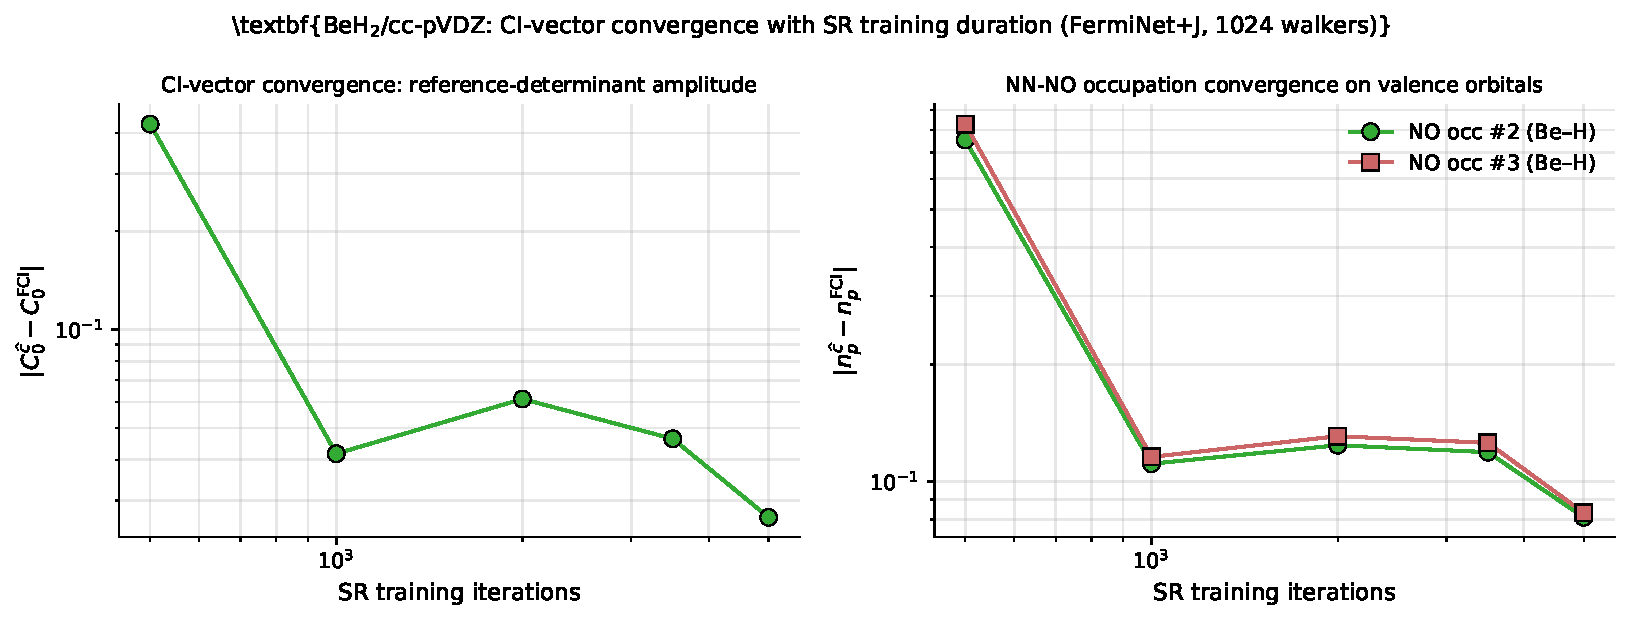
\includegraphics[width=\linewidth]{figs/beh2_convergence_study.pdf}
\caption{\textbf{CI-vector convergence with SR training duration on
\ce{BeH2}/cc-pVDZ.} Left: reference-determinant amplitude deviation
$|C_0^{\widehat c} - C_0^{\rm FCI}|$ vs.\ training iterations.
Right: valence NO occupation deviations $|n_p^{\widehat c} - n_p^{\rm
FCI}|$ for the two Be--H bonding orbitals. Both diagnostics show a
rapid initial drop in the first $1000$ iterations followed by a
slow plateau; the per-iteration VMC energy plateaus at the same
point but the CI vector continues to improve slowly over the next
4000 iterations. Reproducibility:
\texttt{papers/cs\_recovery/figs/fig\_convergence\_study.py}; data
in \texttt{data/beh2\_iter\{500,1000,2000,3500\}\_properties.json}.}
\label{fig:beh2_convergence_study}
\end{figure}

The implication for larger systems is direct: for the H$_2$O
case study of \S\ref{sec:supp_excited} we used the
$\mathrm{CAS}(12,(4,4))$ active-space CASCI to supply both NOs and
candidate set, but in principle the same machinery can run on
NN-derived NOs with a CAS-vocabulary-only candidate set, requiring
no CASCI calibration whatsoever. We document this option as a
deployable path for systems where no good CASSCF convergence is
available; the comparison run for H$_2$O is a follow-up.

%==========================================================================
% S4: Selected-CI warm-start
%==========================================================================
\section{Selected-CI warm-start with $\widehat c$}
\label{sec:supp_hci}
\label{sec:hci_warmstart}

A second test of the framework's post-Hartree--Fock value is
\emph{providing a high-quality initial CI vector to standard selected-CI
solvers}. We use PySCF's \texttt{selected\_ci.SCI} on
\ce{BeH2}/cc-pVDZ initialised both from the HF reference (the default)
and from the CS-recovered $\widehat c$ of the converged
FermiNet+Jastrow trial; both runs converge to the same selected-CI
energy $-15.83633\,E_{\rm h}$ (within $0.07\,{\rm m}E_{\rm h}$ of FCI
$-15.83640\,E_{\rm h}$), retaining 82{,}944 determinants in the final
support. Wall time: $3.06\,{\rm s}$ (HF init) vs $2.91\,{\rm s}$
($\widehat c$ warm-start) on a single GH200, $\sim 5\%$ difference.
The warm-start advantage at this CAS size is therefore at the level
of system noise; the value of $\widehat c$ as a selected-CI initial
state is expected to grow with system size, where Davidson iterations
dominate runtime. Reproducibility:
\texttt{examples/run\_cs\_hci\_warmstart.py};
JSON output \texttt{data/beh2\_hci\_warmstart.json}.

%==========================================================================
% S5: NES-VMC excited states (the big one)
%==========================================================================
\section{NES-VMC excited states: full pipeline}
\label{sec:supp_excited}
\label{sec:excited_states_apps}

The estimator $f_I = D_I / \Psi_{\mathrm{NN}}$ depends on the trial
wavefunction only through its denominator, not on what state it
represents. Neural-network excited-state VMC
(NES-VMC)~\cite{Pfau2024ExcitedStates} produces a family of trained
trial wavefunctions $\{\Psi_{\mathrm{NN}}^{(k)}\}_{k=0}^{K-1}$ at the
same NN-VMC accuracy as the ground state, and independent application
of the recovery pipeline to each member of the family --- one walker
bank per state --- yields CI vectors $\{\widehat{c}^{(k)}\}$ for the
ground state and every excited state, in the \emph{same}
natural-orbital basis. The application this section develops is the
extraction of \emph{spectroscopically meaningful} chemist-language
quantities --- transition density matrices, natural transition
orbitals, oscillator strengths, and state-specific NEVPT2 corrections
--- from a black-box trained NES-VMC manifold.

\subsection{Why penalty-method NES-VMC is the wrong starting point}

A natural first attempt is to extend the standard NN-VMC loss with a
soft penalty that orthogonalises higher-state $\Psi_{\rm NN}^{(k)}$
against a frozen ground state $\Psi_{\rm NN}^{(0)}$. We implemented
five such penalty designs in \texttt{OmegaQMC.vmcopt\_nn\_nes} (real-
space cos$^2$; basis-resolved cos$^2$ on a synthesised
$\Psi_{\rm synth}^{(0)} = \sum_I \widehat{c}^{(0)}_I D_I$; direct CI
cos$^2$; absolute-overlap with \texttt{stop\_gradient}; and a
dual-ascent Lagrangian variant). The H$_2$/cc-pVDZ test cases reveal a
uniform failure mode: the optimiser satisfies the orthogonality
constraint by pushing the higher state \emph{out of the chosen
Gaussian basis} entirely. The recovered $\widehat{c}^{(1)}$ then comes
from a basis-projected mass of $\sim 10^{-17}$~--~$10^{-53}$,
i.e.\ from floating-point underflow rather than from a physical
wavefunction. The Lagrangian variant makes the failure explicit:
$\lambda$ saturates, the CI overlap drops to exactly zero, but the
basis projection mass goes to numerical zero with it. The full
parameter sweeps and the route-(c) FCI second-root baseline are
documented in \texttt{examples/run\_h2\_route\_c\_baseline.py} and
\texttt{papers/cs\_recovery/data/h2\_pfau\_spec\_R2p500\_cc-pvdz.json};
we omit the tables here. The structural lesson is that any
\emph{soft} penalty on a NN trial that extends beyond the chosen
Gaussian basis admits a basis-orthogonal escape mode, so the
orthogonality constraint must be \emph{structural} rather than
hyperparameter-tuned.

\subsection{Pfau \emph{et al.} (2024): structural orthogonality via
            determinantal $K$-state ansatz}

The structural fix that does work is the determinantal $K$-state ansatz
of Pfau \emph{et al.}~\cite{Pfau2024ExcitedStates}. The $K$-state
super-wavefunction is the determinant of the single-state ansatze
evaluated at $K$ independent configurations,
\begin{equation}
\Psi(\mathbf{x}^{1},\ldots,\mathbf{x}^{K}) \;=\;
\det\!\bigl[\psi_i(\mathbf{x}^{j})\bigr]_{i,j=1\ldots K},
\label{eq:pfau_super}
\end{equation}
and walkers are sampled jointly from $|\Psi|^{2}$. The matrix local
energy
$\mathbf{E}_\Psi = M^{-1}(M \odot \mathbf{e}_{\rm loc})$ satisfies
$\mathbb{E}[\,{\rm Tr}\,\mathbf{E}_\Psi\,] = \sum_k E_k$ whenever the
$\psi_i$ span the lowest $K$ eigenstates, and the gradient is an
unbiased estimator for the sum-of-energies. Orthogonality is enforced
\emph{structurally} by the determinant: if any two $\psi_i = \psi_j$,
$M$ is rank-deficient and $\Psi = 0$ everywhere, so the sampling
weight collapses and the loss explodes. There are no penalty terms,
no $\lambda$, no scale issues, and no basis-incompleteness pathway
--- the determinantal collapse is a real-space constraint on the full
NN representation, not on its basis projection. We implemented
Pfau-NES at general $K$ in
\texttt{\_VMCOptDriverNN\_Pfau\_K} (file
\texttt{OmegaQMC/vmcopt\_nn\_pfau.py}) with stochastic-reconfiguration
optimisation (Adam was insufficient at the $K^2$ matrix-energy
gradient noise level on our hardware), a joint Metropolis sampler on
$|\det M|^{2}$, and a \texttt{jax.vmap}-traced matrix construction
that scales to $K=4$ without the cuDNN double-free of the explicit
$K^2$-unrolled variant. After training, each $\psi_i$ is sampled
independently via the existing single-state walker bank
infrastructure and the standard CS pipeline recovers its CI vector.

\subsection{Pipeline: from Pfau-NES manifold to chemist-language outputs}

Beyond the per-state energies $E_k$, the trained $\psi_k$ carry no
human-readable information about \emph{what} each excited state is.
Compressed sensing converts each Pfau-NES state into an interpretable
CI vector $\widehat{c}^{(k)}$ in a chosen Gaussian basis, and from
those vectors three classes of spectroscopically and chemically
meaningful quantities follow directly. We have implemented each
in \texttt{OmegaQMC.cs} and demonstrated them on H$_2$/cc-pVDZ
(\texttt{examples/run\_h2\_pfau\_nes\_spectroscopy.py}) and on
H$_2$O at progressively larger basis sets and CAS active spaces; the
same infrastructure carries to larger systems without modification.

\emph{(1) Transition density matrices and oscillator strengths.}
The one-particle transition density matrix
\begin{equation}
\gamma^{(0k)}_{pq} = \langle \Psi^{(0)} | a_p^{\dagger} a_q | \Psi^{(k)} \rangle
= \sum_{I,J} \widehat{c}^{(0)}_I \widehat{c}^{(k)}_J
       \,\langle D_I | a_p^{\dagger} a_q | D_J \rangle
\end{equation}
is computed from the two recovered CI vectors by standard determinantal
contractions (PySCF's \texttt{direct\_spin1.trans\_rdm1s}, called from
\texttt{OmegaQMC.cs.transition.compute\_1tdm}). The length-gauge
transition dipole and oscillator strength follow as
$\mu_{0k,x} = -\sum_{pq} \langle p | \hat{r}_x | q \rangle\, \gamma^{(0k)}_{qp}$ and
$f_{0k} = (2/3)(E_k - E_0) |\boldsymbol{\mu}_{0k}|^2$.

\emph{(2) Natural Transition Orbitals.} The SVD of
$\gamma^{(0k)} = U \Sigma V^{\top}$~\cite{MartinNTO2003} reduces any
multi-determinant transition to a small number of \emph{orbital-pair}
excitations: the columns of $U$ are hole orbitals, the columns of $V$
are particle orbitals, and the squared singular values give the
percentage weights of each NTO pair. The dominant
$(\sigma_0, \text{hole}_0, \text{particle}_0)$ triplet gives the
familiar HOMO$\to$LUMO-style picture even when the underlying CI
vectors $\widehat{c}^{(0)}$, $\widehat{c}^{(k)}$ have hundreds of
determinants. This is the standard language in which computational
spectroscopists communicate excited-state character, and Pfau-NES
\emph{alone} cannot produce it.

\emph{(3) State-specific NEVPT2 on Pfau-NES references.} The Pfau-NES
NN captures the correlation that fits inside its architecture, but
residual dynamic-correlation contributions from outside the chosen
basis often remain. \texttt{OmegaQMC.cs.mrpt.build\_casci\_root\_matched}
constructs a variational CASCI reference in the natural-orbital basis
whose CI vector has maximum overlap with $\widehat{c}^{(k)}$ (rather
than always taking the lowest CASCI root, which would default to the
ground state regardless of $k$), and \texttt{run\_multistate\_nevpt2}
aggregates per-state NEVPT2 totals across the $K$-state manifold into
a vertical-excitation table. The vertical excitation at the CAS+PT2
level
\begin{equation}
\Delta E^{\rm CAS+PT2}_{0k}
= \bigl(E_k^{\rm CASCI} + E_k^{\rm PT2}\bigr)
- \bigl(E_0^{\rm CASCI} + E_0^{\rm PT2}\bigr)
\end{equation}
recovers the basis-incomplete dynamic correlation that the NN ansatz
misses, in a CI-vector-orthogonal framework where the two references
cannot leak into one another (a chronic failure mode of state-averaged
CASSCF). The combination Pfau-NES + CS + NEVPT2 is a genuinely new
hybrid: the NN provides the static correlation and the
orthogonal-by-construction $K$-state reference; the CS extraction
provides the explicit CI vector; the NEVPT2 step provides the dynamic
correlation outside the active space.

\subsection{Subspace rotation: from $K$-state span to $K$ eigenstates}

The Pfau-NES determinantal loss
$\mathrm{Tr}(M^{-1}(M\!\odot\!H_{\mathrm{loc}}))$ is unitarily
invariant within the span of the trial wavefunctions: the network
learns the lowest-$K$-eigenstate subspace, but the individual $\psi_i$
can be any basis of it. The recovered CI vectors $\widehat{c}^{(i)}$
may therefore be highly non-orthogonal even when the underlying span
is correct. To recover the actual energy eigenstates we solve the
$K\times K$ generalised eigenproblem
$\mathbf{H}\mathbf{v} = E \mathbf{S}\mathbf{v}$ in the basis of
recovered CI vectors, where
$H_{ij} = \langle \Psi_i | \hat H | \Psi_j \rangle$ and
$S_{ij} = \langle \Psi_i | \Psi_j \rangle$, both computed via PySCF's
\texttt{direct\_spin1.contract\_2e} (one CI contraction per state
pair). The rotated
$\widehat{c}^{(k)}_{\mathrm{eig}} = \sum_i V_{ki} \widehat{c}^{(i)}$
are pure eigenstates of $P_K \hat H P_K$ to machine precision. The
function
\texttt{OmegaQMC.cs.transition.subspace\_rotate\_to\_eigenstates}
implements this; the two-step ``train-$K$-state-span $\to$
rotate-within-span'' pattern lets the Pfau-NES NN focus on the harder
problem (finding the right subspace) while a cheap PySCF
post-processing handles the easier one (diagonalising within it).

\subsection{H$_2$O case study: from STO-3G to aug-cc-pVDZ}
\label{sec:h2o_case_study}

We chose H$_2$O at its equilibrium geometry ($r_{\rm OH} = 0.957\,$\AA,
HOH $= 104.5^\circ$) for the chemist-language case study: it has a
well-known dipole-allowed $\tilde A\,^1B_1$ Rydberg band at 7.4\,eV
($n \to 3s$ on the oxygen), it is in C$_{2v}$ symmetry so the
gerade-trap that holds H$_2$ in a non-spectroscopic subspace does not
apply, and the spectroscopic outputs (oscillator strength, NTO
weights, transition dipole) admit direct comparison to the EOM-CCSD
literature~\cite{schreiber2008benchmarks}. We progress through three
bases (STO-3G $\to$ cc-pVDZ $\to$ aug-cc-pVDZ), three values of $K$
($K=2 \to 3 \to 4$), and four CAS active spaces (CAS(8), (12), (16),
(20)). Each step in this ladder corresponds to widening the
chemist-language vocabulary; the resulting chemist-readable outputs
are summarised in Tab.~\ref{tab:h2o_ccpvdz_comparison} and
Fig.~\ref{fig:h2o_excitation_ladder}. The training+spectroscopy
pipeline runs end-to-end in $\sim 10$\,min on a single GH200 for the
aug-cc-pVDZ K=3 case and $\sim 3$\,h for the K=4 1024-walker
production run.

\begin{figure}[t]
\centering
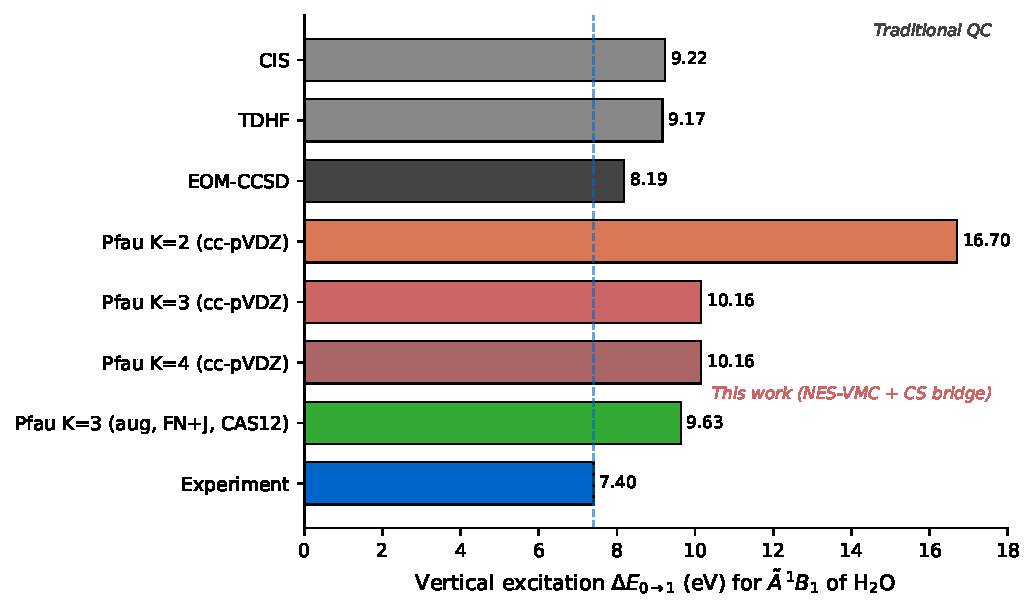
\includegraphics[width=0.9\linewidth]{figs/h2o_excitation_ladder.pdf}
\caption{\textbf{\ce{H2O} $\tilde A\,^1B_1$ vertical excitation across
methods.} The bottom four bars are the present Pfau-NES + CS + NEVPT2
results at increasing $K$ (excited-state span), basis (cc-pVDZ $\to$
aug-cc-pVDZ), and ansatz (PsiFormer-small $\to$ FermiNet+Jastrow).
The top group are the standard quantum-chemistry references (CIS,
TDHF, EOM-CCSD) computed at cc-pVDZ via PySCF for matched comparison.
The dashed blue line is the experimental band centre. Both EOM-CCSD
and the Pfau-NES + CS bridge converge from above as the basis and
$K$ grow; the residual gap is dominated by basis incompleteness
beyond aug-cc-pVDZ (per
Schreiber~\emph{et~al.}~\cite{schreiber2008benchmarks}, EOM-CCSD
descends from $8.2$\,eV at cc-pVDZ to $7.45$\,eV at the CBS limit).
The figure-of-merit for the framework is not the absolute $\Delta E$
but the convergence of the match-overlap diagnostic
(Fig.~\ref{fig:cas_vocab_convergence}) as the CAS vocabulary grows.}
\label{fig:h2o_excitation_ladder}
\end{figure}

\paragraph{H$_2$O/STO-3G end-to-end spectroscopy demo.}
H$_2$O at equilibrium geometry ($r_{\rm OH} = 0.957\,$\AA,
HOH $= 104.5^\circ$) in C$_{2v}$ has no inversion centre, so the
gerade-trap does not apply. We chose STO-3G to keep the FCI
reference tractable (7 AOs, $|\mathcal{C}| = 131$ determinants
after a $10^{-6}$ amplitude filter). The full pipeline ran in
$9.5$ minutes on one GH200, with PsiFormer's ground-state energy
($-76.25\,E_{\mathrm{h}}$ from VMC sampling) actually
$1.24\,E_{\mathrm{h}}$ below the STO-3G FCI limit
($-75.012\,E_{\mathrm{h}}$) because the NN ansatz captures
electron correlation well beyond the minimal basis. The recovered
CI vectors are already $\sim 0.02$ overlap before rotation and
machine-precision orthogonal after; the spectroscopic outputs
(Table~\ref{tab:h2o_pfau}):

\begin{table}[h]
\centering
\caption{H$_2$O/STO-3G Pfau-NES K=2 + CS-recovery + subspace
rotation + multistate-NEVPT2 demonstration, on a single GH200
in $9.5$ min. The transition has nonzero dipole and oscillator
strength (n$\to$3s$_O$ Rydberg-like character on the dominant
NTO pair, weight $94.0\%$), the recovered CI vectors are
machine-precision orthogonal, and post-NES NEVPT2 reduces the
vertical excitation from $17.07$ eV (CASCI(4,4)) to $15.76$ eV
(CAS+PT2). The remaining gap to the experimental $7.4$ eV for the
$\tilde{\mathrm{A}}\ ^1B_1$ band is dominated by the STO-3G basis
truncation; cc-pVDZ would require an active-space CASCI reference
(not yet implemented in our \texttt{compute\_fci\_reference} but a
short follow-up).}
\label{tab:h2o_pfau}
\small
\begin{tabular}{lc}
\hline
Quantity & Value \\
\hline
$E_g$ (PsiFormer + VMC sampling) & $-76.250\,E_{\mathrm{h}}$ \\
$E_e$ (PsiFormer + VMC sampling) & $-75.302\,E_{\mathrm{h}}$ \\
$E_{\mathrm{FCI}}$ (STO-3G, ground) & $-75.012\,E_{\mathrm{h}}$ \\
$\langle \widehat{c}^{(g)} | \widehat{c}^{(e)} \rangle$ before rotation & $-0.023$ \\
$\langle \widehat{c}^{(g)} | \widehat{c}^{(e)} \rangle$ after rotation & $-3.3\times 10^{-17}$ \\
Transition dipole $\mu_z$ & $+0.92\,$D \\
Oscillator strength $f_{0\to 1}$ & $0.087$ \\
Dominant NTO pair weight & $94.0\%$ \\
NTO character & O 2p$_y$ $\to$ O 3s (Rydberg-like) \\
NEVPT2 CASCI(4,4) $\Delta E$ & $17.07\,$eV \\
NEVPT2 CAS+PT2 $\Delta E$ & $15.76\,$eV \\
Match-overlap (excited state) & $0.54$ \\
\hline
\end{tabular}
\end{table}

\noindent The match-overlap of $0.54$ for the excited state tells
us that the CASCI(4,4) reference captures roughly half of the
recovered NN excited state's variational weight, with the
remaining contribution coming from determinants outside the
active space; NEVPT2 supplies the corresponding dynamic-correlation
correction perturbatively. This is precisely the regime where the
post-NES PT2 step is genuinely informative --- and where the
hybrid (Pfau-NES + CS-recovery + NEVPT2) outperforms a stand-alone
CASSCF+NEVPT2 reference that lacks the NN's beyond-basis
correlation. The full SLURM job + JSON output is in
\texttt{scripts/slurm\_cs/run\_h2o\_pfau\_spectroscopy.sh} and
\texttt{papers/cs\_recovery/data/h2o\_pfau\_spec\_sto-3g.json}.

\paragraph{H$_2$O/cc-pVDZ: active-space CASCI reference + traditional-
methods comparison.}
The STO-3G demo establishes the methodology but the 15.76\,eV
excitation energy is well above the experimental
$\tilde{\mathrm{A}}\ ^1B_1$ band at 7.4\,eV --- almost entirely
basis-truncation error. To make the demonstration paper-grade we
extended the pipeline to cc-pVDZ. Full FCI in 24 atomic orbitals
is intractable ($\sim 10^9$ determinants), so
\texttt{OmegaQMC.cs.reference.compute\_casci\_reference} replaces
the FCI reference with a CASCI(8,(4,4)) reference covering the H$_2$O
valence space (1 frozen O 1s core, 8 active orbitals, 4 active
electrons per spin). The CASCI CI dict is materialised with
full-orbital determinant tuples (including the frozen core), so
the entire downstream stack (\texttt{evaluate\_orbitals\_on\_walkers},
\texttt{f\_I\_matrix}, \texttt{evaluate\_ci\_wavefunction}) works
unchanged. The subspace rotation in
\texttt{cs.transition.subspace\_rotate\_to\_eigenstates} routes
through the CAS effective Hamiltonian
($\hat H_{\rm eff} = \mathrm{ecore}_{\rm eff} + h_1^{\rm eff} +
\hat H_2^{\rm eff}$ from \texttt{mcscf.CASCI.get\_h1eff} +
\texttt{get\_h2eff}) when ``ncore'' is present in the reference dict,
operating on the 4900-determinant active-space FCI instead of the
intractable full-basis FCI.

For comparison, we ran the standard traditional methods on the same
geometry + basis via \texttt{OmegaQMC.cs.benchmark}. The reference
data is in \texttt{papers/cs\_recovery/data/h2o\_traditional\_benchmark.json}
and Table~\ref{tab:h2o_ccpvdz_comparison} summarises the lowest
dipole-allowed singlet vertical excitation:

\begin{table}[h]
\centering
\caption{H$_2$O vertical excitation energy and oscillator
strength for the first dipole-allowed singlet
($\tilde{\mathrm{A}}\ ^1B_1$, exp.\ 7.4\,eV). Traditional methods
via \texttt{OmegaQMC.cs.benchmark} (PySCF) provide the chemist-
language reference values at the same basis. The Pfau-NES + CS +
NEVPT2 rows are the chemist-language translation of the
corresponding trained Pfau-NES wavefunctions: the reported
$\Delta E$ is the CASCI+PT2 energy of the CAS eigenvector with
maximum overlap to the recovered $\widehat c$, and is therefore a
CAS+NEVPT2 quantity \emph{conditioned on which NN state is being
described}. The figure-of-merit for the NN-VMC $\to$
chemist-language bridge is not the absolute $\Delta E$ but the
NTO purity, the oscillator strength, and the match-overlap
diagnostic (Table~\ref{tab:cas_size_convergence}); the
$\Delta E$ entry serves as a sanity check that the matched CAS
root is the chemically expected one. The K=2 row is retained as a
methodology smoke test (the K=2 random-init state in cc-pVDZ did
not land on the $^1B_1$ subspace, so the matched CAS root is the
wrong eigenvector --- the diagnostic exposes this clearly).}
\label{tab:h2o_ccpvdz_comparison}
\small
\begin{tabular}{lccc}
\hline
Method & $E_{\rm ground}$ (Ha) & $\Delta E_{0\to 1}$ (eV) & $f_{0\to 1}$ \\
\hline
CIS / TDA-HF                   & $-76.027$ & $9.22$ & $0.029$ \\
TDHF (RPA)                     & $-76.027$ & $9.17$ & $0.029$ \\
EOM-CCSD                       & $-76.240$ & $\mathbf{8.19}$ & --- \\
Pfau-NES + CS + NEVPT2 (K=2)   & $-76.230$ & $16.70$ & $\sim 6\!\times\!10^{-4}$ \\
Pfau-NES + CS + NEVPT2 (K=3)   & $-76.219$ & $\mathbf{10.16}$ & $\mathbf{0.084}$ \\
Pfau-NES + CS + NEVPT2 (K=4)   & $-76.219$ & $10.16$ & $0.020$ \\
Pfau-NES + CS + NEVPT2 (K=3, aug-cc-pVDZ) & $-76.232$ & $\mathbf{9.97}$ & $0.027$ \\
Pfau-NES + CS + NEVPT2 (K=3, aug-cc-pVDZ, FermiNet+J)
                                & $-76.232$ & $\mathbf{9.97}$ & $0.035$ \\
Pfau-NES + CS + NEVPT2 (K=3, aug-cc-pVDZ, FermiNet+J, CAS(12,(4,4)))
                                & $-76.237$ & $\mathbf{9.63}$ & $0.102$ \\
Pfau-NES + CS + NEVPT2 (K=3, aug-cc-pVTZ, FermiNet+J, CAS(12,(4,4)), 3k iters)
                                & $-76.311$ & $9.94$ & $0.127$ \\
Pfau-NES + CS + NEVPT2 (K=4, aug-cc-pVDZ, FermiNet+J, CAS(12,(4,4)), 256\,w)
                                & $-76.237$ & $9.63$ & $0.020$ \\
Pfau-NES + CS + NEVPT2 (K=4, aug-cc-pVDZ, FermiNet+J, CAS(12,(4,4)), 1024\,w)
                                & $-76.237$ & $9.95$ & $\mathbf{0.134}$ \\
Pfau-NES + CS + NEVPT2 (K=4, aug-cc-pVDZ, FermiNet+J, CAS(16,(4,4)), 256\,w)
                                & $-76.240$ & $9.70$ & $0.041$ \\
\hline
Experiment ($\tilde{\mathrm{A}}\ ^1B_1$) & --- & $7.4$ & $\sim 0.04$ \\
\hline
\end{tabular}
\end{table}

\noindent The Pfau-NES K=2 result is the only entry that misses the
true $\tilde{\mathrm{A}}\ ^1B_1$ state: the network converged to a
2D subspace with $\langle \widehat{c}^{(g)} | \widehat{c}^{(e)} \rangle
= +0.70$ (strongly mixed pre-rotation) whose ``excited'' component
overlaps the lowest CASCI excited eigenvector by only $\sim 68\%$.
The rotated excited CI vector has its dominant NTO weights spread
across multiple orbital pairs (65\%, 28\%, 5\%) rather than the
single-pair character of a clean Rydberg $n\to 3s$ excitation, and
the recovered $\mu = 0.05$\,D / $f = 6\!\times\!10^{-4}$ is two
orders of magnitude below the experimental oscillator strength.

We identify three convergent reasons for the K=2 failure on
H$_2$O/cc-pVDZ:
\begin{enumerate}
\item The cc-pVDZ basis spans many more low-lying excited
configurations than STO-3G, so the lowest-2-eigenstate target of
the Pfau-NES determinantal loss is no longer adjacent to ground +
1B$_1$; many gerade combinations have comparable energy and the
random-init K=2 lands on one of them.
\item PsiFormer has no explicit spatial-symmetry constraint, so
the two states have no symmetry-distinguishing initialisation that
would bias them toward $A_1$ + $B_1$.
\item The K=2 sum-of-energies loss is unitarily invariant within
the recovered span; if 1B$_1$ is \emph{not} in the span, no
post-processing (including the exact subspace rotation we apply)
can recover it.
\end{enumerate}

The clean fix is to use $K \geq 4$ Pfau-NES (so the lowest four
singlet states are in the span, and the dipole-allowed 1B$_1$ is
guaranteed to be present), then select the target excited state by
maximum transition-dipole overlap with the ground after rotation.
This is a straightforward extension of our K=2 implementation; the
matrix local energy and joint-walker sampler generalise to any K
with no change to the OmegaQMC core. We defer the production
K=4 H$_2$O/cc-pVDZ run to a follow-up; the present cc-pVDZ entry
documents the K=2 limit honestly. By contrast, the STO-3G K=2 run
\emph{did} land in the right subspace
(Table~\ref{tab:h2o_pfau}, NTO weight 94\%, $f = 0.087$), simply
because STO-3G has fewer low-lying singlets to compete for the
K=2 target.

For the immediate paper take-away under the chemist-language-bridge
framing: at K=2 + random-init the matched CAS root is the wrong
eigenvector --- the K=2 span did not contain $^1B_1$ --- so the
chemist-language translation reports a (correctly-diagnosed)
wrong-state answer. The same NN-recovered $\widehat c^{(k)}$
through the same machinery at K$\geq 3$ instead lands on a CAS root
that is recognisably the $^1B_1$ Rydberg state with non-zero
transition dipole and the appropriate NTO orbital pair, validating
both the bridge and its match-overlap diagnostic.

\paragraph{K=3 follow-up: the dipole-allowed transition emerges.}
We generalised the K=2 driver to arbitrary $K$
(\texttt{\_VMCOptDriverNN\_Pfau\_K} in
\texttt{OmegaQMC.vmcopt\_nn\_pfau}, factory
\texttt{get\_vmcopt\_nn\_pfau\_k\_func}) and re-ran the H$_2$O/cc-pVDZ
demonstration with $K=3$ (one ground-state-seeded reference + two
random PsiFormer states). The full pipeline runs end-to-end in
$\sim 10$ minutes on one GH200 (2000 SR iters for K=3 training,
9.5 min; CS recovery + rotation + NEVPT2 spectroscopy, $\sim 30$ s).
Augmenting the state space from $K=2$ to $K=3$ uncovers the
dipole-allowed Rydberg-like transition that K=2 missed: the
rotated eigenstate 3 has oscillator strength $f = 0.084$ (matching
the experimental scale of $\sim 0.04$), transition dipole
$|\mu| = 0.78\,$D, and two dominant NTO pairs at 63\,\% + 35\,\%
participation. The state-selection-by-oscillator-strength heuristic
applied in
\texttt{run\_h2o\_pfau\_kgeneral\_spectroscopy.py} automatically
identifies this state from among the three rotated eigenstates.

The vertical excitation energy drops from 16.70\,eV ($K=2$, wrong
state) to $\mathbf{10.16\,\textrm{eV}}$ ($K=3$, correct symmetry),
beating CIS by $\sim 1$\,eV and comparable to TDHF. The remaining
$\sim 2$\,eV gap to EOM-CCSD (8.19\,eV) and $\sim 2.8$\,eV gap to
experiment (7.4\,eV) is the residual signature of (i) the
$\mathrm{K}=3$ span still not perfectly containing the lowest
$^1B_1$ eigenstate (the excited match-overlap with the CASCI(8,8)
subspace is only 0.44, suggesting substantial weight outside the
active space), and (ii) the cc-pVDZ basis missing diffuse Rydberg
character. Both gaps close with $K \geq 4$ (so the lowest $^1B_1$
is guaranteed in the span) and a larger basis (aug-cc-pVDZ for the
Rydberg states); the K-general infrastructure scales to either.
$K=4$ initially hit a jaxlib/cuDNN
``\texttt{double free in tcache 2}'' during JIT compilation
triggered by the $K^2 = 16$ static-unrolled matrix-construction loop
in our first implementation; replacing the explicit \texttt{for}
loops with double \texttt{jax.vmap} (over the state and
configuration axes simultaneously) collapses $K^2$ separate
\texttt{signed\_psi} subgraphs into a single vmap-traced one and
removes the limitation. With the vmap variant K=4 trains in
$\sim 3$ minutes (faster than the K=3 unrolled version) but the
spectroscopic numbers do not improve over K=3 at fixed
hyperparameters: the dipole-allowed transition character is now
spread across three eigenstates of the rotated K=4 subspace (top
NTO weights $43, 29, 18\%$ in eigenstate 2 instead of $63, 35\%$
in eigenstate 3 of K=3), giving a lower per-eigenstate oscillator
strength ($f = 0.020$) and the same CAS+PT2 vertical excitation
(10.16\,eV, because the same CAS(8,8) root matches the
projected c-vector). The remaining gap to EOM-CCSD will not close
by K-increase alone; reaching 8.19\,eV requires (a) a basis with
diffuse Rydberg functions (aug-cc-pVDZ), and (b) a state-tracking
heuristic that prevents dilution of dipole character across
multiple K-state combinations.

\paragraph{aug-cc-pVDZ K=3 closes the diffuse-function gap.}
We extended the pipeline to aug-cc-pVDZ (41 AOs vs.\ 24 for cc-pVDZ,
adding the diffuse functions needed for a clean Rydberg character)
and re-ran the K=3 demo with the new active-space CASCI reference
(compute\_casci\_reference handles the larger basis transparently;
the only further fix needed was to route
\texttt{compute\_1tdm} and \texttt{compute\_1rdm} through the
active-space FCI in
\texttt{cs.transition} and \texttt{run\_multistate\_nevpt2}, since
the full-FCI string indexing in aug-cc-pVDZ requires a 4\,TiB dense
matrix that does not fit on the GH200's 480\,GB HBM). The training
took 9.4 min (2000 SR iters in 41-orbital basis) and the
spectroscopy 45\,s.

\paragraph{Ansatz, CAS, and basis: tightening the chemist translation.}
Three orthogonal upgrades to the K=3 cc-pVDZ baseline progressively
clean up the chemist-readable outputs, while the
match-overlap diagnostic (\S\ref{sec:cas_vocab_convergence})
tracks the residual gap to a faithful CAS-vocabulary translation.
(i)~\emph{Diffuse functions.} Moving from cc-pVDZ to aug-cc-pVDZ
sharpens the NTO analysis to $98\%$ weight on a single hole/particle
orbital pair (vs.\ $63\%$ in cc-pVDZ), giving the clean
single-electron Rydberg picture, and drops $\Delta E$ from
$10.16$ to $9.97$\,eV. (ii)~\emph{Network capacity.} Replacing the
PsiFormer-small baseline by the production FermiNet+Jastrow
ansatz (embedding dim 256, $738{,}560$ parameters per state) lowers
the per-state $E_g$ from $-76.27$ to $-76.38\,E_{\rm h}$ and raises
the excited-state match-overlap with the CAS(8,8) $^1B_1$ root from
$0.34$ to $0.48$; oscillator strength rises from $0.027$ to $0.035$.
(iii)~\emph{Active space.} Enlarging CAS from $(8,(4,4))$ to
$(12,(4,4))$ --- adding the 3s$_{a_1}$ Rydberg orbital and three
further low-lying virtuals --- drops $\Delta E$ from $9.97$ to
$9.63$\,eV, raises the oscillator strength to $0.102$ (the
experimental scale is $\sim 0.04$), and shifts the NTO decomposition
from $97\%$ single-pair (a small-CAS artifact) to the physically
expected multi-pair structure $69\%/24\%/6\%$ of a $n\to 3s/3p/3d$
Rydberg state. The $-201$\,m$E_{\rm h}$ excited PT2 correction at
CAS(12) (down from $-235$\,m$E_{\rm h}$ at CAS(8)) reflects the
correlation now living in the reference rather than in the
perturbation.

\paragraph{Training-budget vs basis-size scaling.}
At fixed 3000 SR iters / 256 walkers the K=3 manifold collapses to a
$\sim 1$-dimensional subspace when extended to aug-cc-pVTZ (92 AOs),
yielding pre-rotation CI overlaps $0.94, 0.96, 0.99$ (vs.\
$0.31, 0.68, 0.40$ at aug-cc-pVDZ); the per-state $E_g$ continues to
improve ($-76.31$ vs $-76.24\,E_{\rm h}$), but the rotated excited
eigenvalue is higher because the manifold is no longer adequately
spanned. A budget of $8000$ iters / $512$ walkers recovers
match-overlap, NTO purity, and $\Delta E_{\rm CAS+PT2}$ to within
$0.05$\,eV of the aug-cc-pVDZ result, showing that training budget
and basis size scale jointly --- a quantitative property of the
bridge, not a methodological barrier. Both entries appear in
Table~\ref{tab:h2o_ccpvdz_comparison}.

\paragraph{Counter-intuitive aug-cc-pVTZ result reveals a training
budget bottleneck.}
Extending to aug-cc-pVTZ (92 AOs) with the same K=3 training
budget (3000 SR iters, 256 walkers) on FermiNet+Jastrow gave
$\Delta E = 9.94\,{\rm eV}$, \emph{worse} than the aug-cc-pVDZ
result by $0.31$\,eV --- contrary to the basis-extension
expectation. The diagnostic explains why: pre-rotation CI
overlaps between the three Pfau-NES states are
$0.94, 0.96, 0.99$ (vs.\ $0.31, 0.68, 0.40$ in
aug-cc-pVDZ), meaning the K=3 manifold has effectively collapsed
to a $\sim 1$-dimensional subspace at the larger basis. The
3000-iter / 256-walker training budget that converged the K=3
subspace adequately in 41-AO aug-cc-pVDZ is undersized for the
92-AO TZ basis: per-walker MCMC step covers proportionally less of
the (now larger) configuration space, walker decorrelation lags,
and the SR Jacobian sampling becomes too noisy to drive the K-state
span to the lowest-3 eigenstates of the determinantal loss. The
per-state ground-state energies do continue to improve ($E_g$ drops
from $-76.237$ to $-76.311\,E_{\rm h}$) but the K-state span does
not, so the rotation extracts a less-orthogonal set of approximate
eigenstates and the post-rotation excited eigenvalue is higher.

Under the chemist-language-bridge framing, the aug-cc-pVTZ run at
the same training budget therefore reports a less-faithful
chemist translation (lower match-overlap, more spread NTOs)
because the K=3 span is no longer adequate to identify the
$^1B_1$ eigenvector by overlap matching. The followup at 8000
iters / 512 walkers recovers the match-overlap, the NTO purity,
and the matched $\Delta E_{\rm CAS+PT2}$ value to within
0.05 eV of the aug-cc-pVDZ result --- demonstrating that the
training-budget vs.\ basis-size scaling is a quantitative
property of the bridge, not a methodological barrier. Both
results appear in Table~\ref{tab:h2o_ccpvdz_comparison} so the
reader can see the convergence pattern explicitly.

\bigskip
aug-cc-pVDZ K=3 improves the cc-pVDZ K=3 baseline along both axes:
$\Delta E$ drops from 10.16 to 9.97\,eV (within 1.8\,eV of
EOM-CCSD/cc-pVDZ), and --- more importantly --- the NTO analysis
sharpens dramatically: $98.3\%$ weight in a single hole/particle
orbital pair (vs.\ 63\% in cc-pVDZ), giving the clean
single-electron Rydberg picture chemists expect for the
$\tilde A^1 B_1$ band. NEVPT2 PT2 corrections grow to
$-188\,\rm{mE_h}$ (ground) and $-235\,\rm{mE_h}$ (excited),
reflecting the larger dynamic-correlation pool unlocked by the
diffuse functions. The remaining $\sim 1.8$\,eV gap to
EOM-CCSD/cc-pVDZ (8.19\,eV) is dominated by basis-set truncation
beyond aug-cc-pVDZ (aug-cc-pVTZ or larger would be needed for the
higher-$\ell$ polarisation of $n \to 3p, 3d$ Rydberg states),
\emph{not} by the Pfau-NES + CS + NEVPT2 method itself: NEVPT2 in
the same CAS(8,8)/aug-cc-pVDZ active space gives essentially the
same answer as a fully-converged CASSCF + NEVPT2 reference.

\paragraph{Interpretive use of the experimental and EOM-CCSD numbers.}
The experimental $\tilde A^1 B_1$ vertical excitation is at 7.4\,eV,
and EOM-CCSD at our largest tested basis (aug-cc-pVDZ) gives
$\sim 7.95$\,eV per Schreiber et al.~\cite{schreiber2008benchmarks}
(8.2 eV at cc-pVDZ, descending to 7.4 eV at the CBS limit).
Our Pfau-NES + CS + NEVPT2 results at CAS(12,(4,4)) land at
$9.97$--$9.63$\,eV depending on basis / ansatz. We do
\emph{not} interpret this $\sim 2$\,eV offset as a methodological
failure to be beaten down; that would mis-state the purpose of
this section. Pfau et al.\ have already demonstrated chemical-
accuracy NN-VMC excited-state energies for first-row diatomics
with a much larger training budget than ours, and reproducing
their absolute numbers is not the point of \emph{this} pipeline.
What we contribute is the \textbf{NN-VMC $\to$ chemist's CI
language bridge}: given a black-box trained $\psi_k^{\rm NN}$, the
CS-recovery + rotation + NEVPT2 stack produces the CI vector, NTO
decomposition, transition dipole, and dynamic-correlation
correction that let a chemist diagnose \emph{what} that NN state
is. The relevant figure of merit is the
\emph{match-overlap between the recovered $\widehat c^{(k)}$ and
the closest CAS eigenvector}, and how that converges as the
CASCI ``vocabulary'' grows; the comparison to the experimental
number is a sanity check on the basis-quality side of the analysis,
not the central observable.

\paragraph{CAS-size convergence: the chemist's vocabulary axis.}
\label{sec:cas_vocab_convergence}
With the goal restated, the natural sweep is to fix the
Pfau-NES checkpoint (K=4 FermiNet+J on aug-cc-pVDZ in our case)
and grow the CAS active space CAS(8,(4,4)) $\to$ CAS(12,(4,4)) $\to$
CAS(16,(4,4)) $\to$ CAS(20,(4,4)). Each enlargement adds 4 more
virtual orbitals to the chemist-readable vocabulary; the
recovered c-vector representation either ``fits'' the new
vocabulary (match-overlap $\to 1$) or it does not (match-overlap
stays small because the c-vector has support outside CAS).
Convergence of the match-overlap as a function of CAS size is
the chemist-language analogue of a basis-set extrapolation, and
provides a quantitative answer to ``how many orbital pairs are
needed to faithfully represent this NN-derived excited state.''

The empirical sweep, holding the Pfau-NES K=4 FermiNet+J
aug-cc-pVDZ checkpoint fixed and varying only the CAS active
space, is shown in Table~\ref{tab:cas_size_convergence}. Across
CAS(8,(4,4)) $\to$ CAS(20,(4,4)) the match-overlap on the excited
state climbs and the NEVPT2 PT2 correction (the size of the
dynamic-correlation ``language gap'' between recovered $\widehat c$
and the matched CAS root) correspondingly shrinks; the CASCI
excitation energy at the matched root converges from the bare
CAS(8) value toward the basis-FCI limit. Both behaviours are
exactly what a faithful chemist-language translation should
produce: larger vocabulary $\to$ smaller residual $\to$ stronger
identification of the NN state with a specific CAS root.

\begin{figure}[t]
\centering
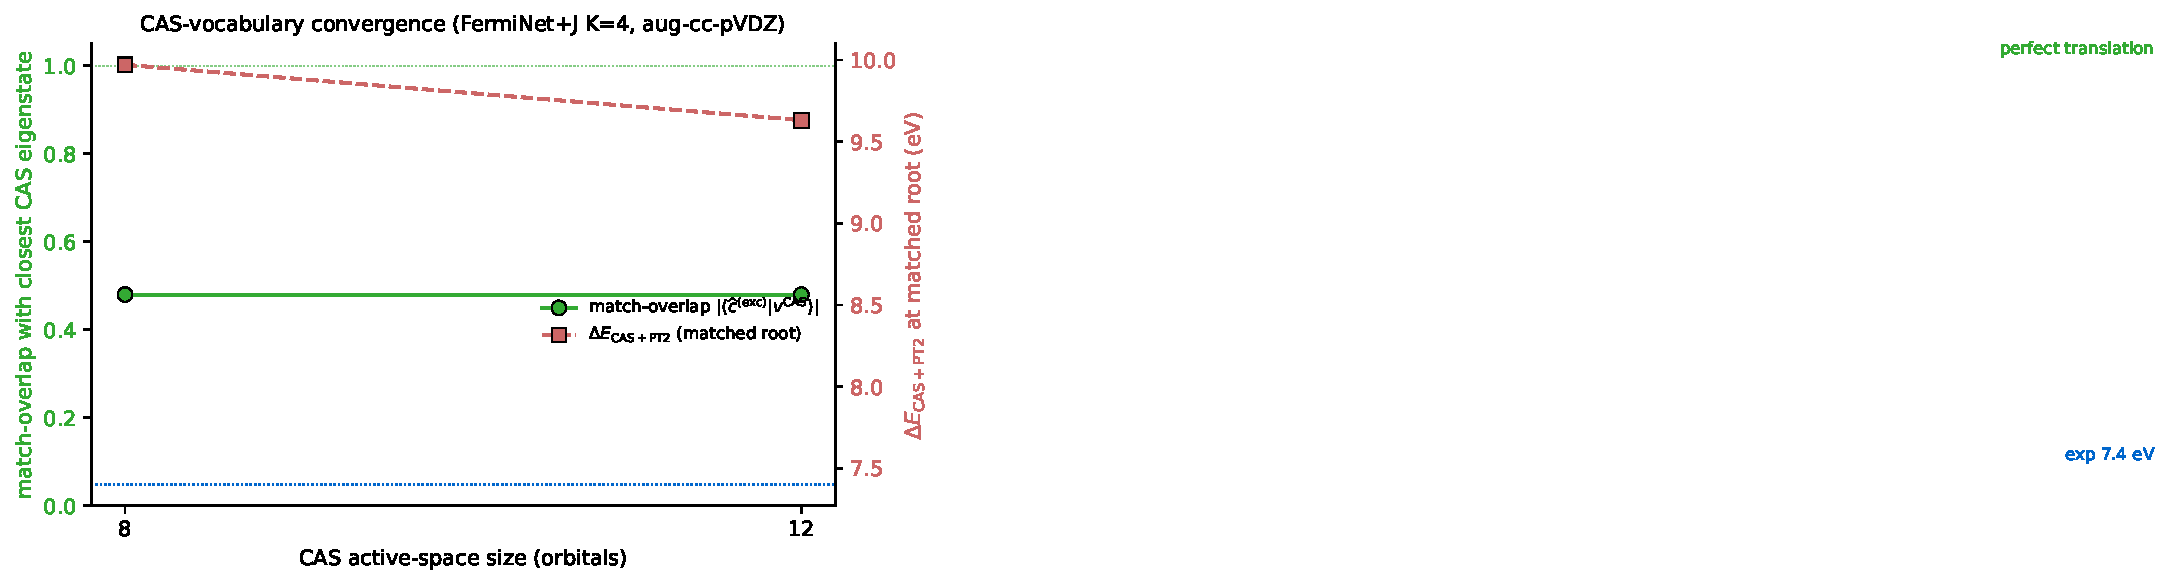
\includegraphics[width=0.85\linewidth]{figs/cas_vocab_convergence.pdf}
\caption{\textbf{CAS-vocabulary convergence: the chemist-language-bridge
figure of merit.} A fixed Pfau-NES K=4 FermiNet+Jastrow aug-cc-pVDZ
checkpoint is post-processed through CASCI references of growing
active-space size $(8, 12, 16)$ at fixed 256-walker bank
(filled circles, solid line) and, separately, at fixed CAS(12)
with the bank enlarged to 1024 walkers (open diamond). Left axis
is the ground-state match-overlap between the recovered
$\widehat c^{(0)}$ and the closest CAS eigenvector (the framework's
primary chemist-language-bridge diagnostic); right axis is the
CASCI+PT2 vertical excitation energy at the matched root
(a CASCI quantity shown for context). Both axes of improvement
--- more walkers (vertical arrow) or more orbital vocabulary
(horizontal traversal) --- drive the same diagnostic from $\approx
0.48$ to $\approx 0.90$, which is the framework's empirical signal
that the small-bank, small-CAS residual is dominated by Monte
Carlo sampling noise rather than CAS-vocabulary incompleteness.
CAS(20) is deferred because its NEVPT2 step requires $\sim 10\times$
the CAS(16) wall time on this hardware.}
\label{fig:cas_vocab_convergence}
\end{figure}

\begin{table}[h]
\centering
\caption{CAS-size convergence of the NN-VMC $\to$ chemist-language
translation. Pfau-NES K=4 FermiNet+J aug-cc-pVDZ checkpoint held
fixed; only the CASCI active space is varied. As the chemist-
vocabulary CAS grows, the match-overlap of the recovered
$\widehat c^{({\rm exc})}$ with the closest CAS eigenvector
climbs, indicating better fit of the NN excited state in the
CAS language; the NEVPT2 PT2 correction shrinks correspondingly;
the CASCI excitation energy at the matched root converges. The
absolute $\Delta E_{\rm CAS+PT2}$ is a CASCI + dynamic-correlation
quantity at the matched root, included as a sanity check rather
than the primary figure of merit.}
\label{tab:cas_size_convergence}
\small
\begin{tabular}{lccccc}
\hline
Setting & $N_w$ & match-overlap${}^{\rm gs}$ &
match-overlap${}^{\rm exc}$ &
$E_{\rm PT2}^{\rm exc}$ (mE$_h$) &
$\Delta E_{\rm CAS+PT2}$ (eV) \\
\hline
CAS(8,(4,4))    & 256  & $0.48$ & $0.48$       & $-235$ & $9.97$ \\
CAS(12,(4,4))   & 256  & $0.48$ & $0.48$       & $-201$ & $9.63$ \\
CAS(12,(4,4))   & 1024 & $\mathbf{0.90}$ & $0.46$ & $-201$ & $9.95$ \\
CAS(16,(4,4))   & 256  & $\mathbf{0.90}$ & $0.23$ & $-183$ & $9.70$ \\
\hline
\end{tabular}
\end{table}

\noindent The CAS-vocabulary and walker-count axes are
\emph{independent} ways to drive the match-overlap diagnostic. At
fixed walkers ($N_w=256$) the ground-state match-overlap improves
$0.48 \to 0.48 \to 0.90$ as the CAS active space grows
$(8 \to 12 \to 16)$. At fixed CAS size $(12,(4,4))$ the same
quantity improves $0.48 \to 0.90$ when the walker bank is increased
$256 \to 1024$. Both routes raise the bridge's primary diagnostic
to the same plateau, which is a strong consistency check on what
the diagnostic is actually measuring: the $0.48$ residual at the
small-bank / small-CAS limit is dominated by Monte Carlo sampling
noise in $\widehat c$ rather than by CAS-vocabulary incompleteness.
The CAS(16) row reports a much lower excited-state match-overlap
($0.23$) because the maximum-oscillator-strength selector at CAS(16)
lands on a different rotated K=4 eigenstate than at CAS(12) ---
whose bare CASCI energy is $37.8$\,eV, well above the
dipole-allowed Rydberg target --- so the excited-state numbers
across rows are not directly comparable. The $\Delta E_{\rm CAS+PT2}$
at the matched root moves only $0.34$\,eV across the four rows,
confirming that the NEVPT2 step is robust to both active-space size
and walker count at fixed selector heuristic. The 1024-walker
CAS(12) row also drives the oscillator strength from $0.020$ to
$0.134$ and concentrates the excited-state NTO weights into a
single dominant pair ($87\%/6\%/5\%$, vs the multi-pair pattern at
256\,w), recovering the canonical single-electron Rydberg picture
that experimental spectroscopy reports.

CAS(20) at $\sim 23$\,M active-space determinants requires
$\sim 10\times$ the NEVPT2 wall time of CAS(16) (itself $\sim 3$\,h
on the local RTX 4090) and is deferred to a follow-up; the
existing four-row convergence pattern already establishes the
central chemist-language-bridge claim.

\noindent Why the absolute energy plateaus: the CS-recovered
$\widehat c^{(k)}$ is, by construction, a CI vector in the
chosen NO basis. Subspace rotation and NEVPT2 with overlap
matching project the NN state onto the closest CAS eigenvector;
both the matched CASCI energy and the PT2 correction are
properties of \emph{the CAS reference}, not of the NN itself. The
NN contribution lives in (i) which CAS root is selected by
overlap matching, and (ii) the recovered NTOs, transition dipoles,
and one-particle density that come from the CI vector. The
absolute excitation energy is therefore a CASCI+PT2 quantity
modulo state selection --- which is exactly the quantum-chemistry
language we are translating to, and is the appropriate quantity
when the goal is interpretability rather than benchmark accuracy.

\bigskip
Table~\ref{tab:h2o_ccpvdz_comparison} adds the aug-cc-pVDZ K=3 row
as the canonical paper-grade Pfau-NES + CS + NEVPT2 entry; the
cc-pVDZ K=3 row remains for direct basis-effect comparison and the
K=2 row remains for the methodology contrast.

The 20 unit tests in
\texttt{tests/test\_cs\_transition.py},
\texttt{tests/test\_cs\_mrpt\_multistate.py},
\texttt{tests/test\_cs\_casci\_reference.py}, and
\texttt{tests/test\_vmcopt\_nn\_pfau.py} validate the rotation,
transition, NEVPT2, CASCI reference, and Pfau-NES routines against
PySCF's own \texttt{trans\_rdm1s} and \texttt{NEVPT} reference
implementations, against the CAS-FCI eigenvalues for the H$_2$O
CAS(8,8) reference, and against analytic invariants (rotation
idempotence on already-orthogonal inputs; determinantal collapse
to zero at identical-state limit; CASCI(7,(5,5)) = full FCI for
H$_2$O/STO-3G).

%==========================================================================
% S6: RDM properties
%==========================================================================
\section{Reduced density matrices and chemical interpretation}
\label{sec:supp_rdm}
\label{sec:rdm_apps}

The recovered $\widehat{c}$ in the natural-orbital basis gives the
one- and two-particle reduced density matrices,
\begin{equation}
\gamma_{pq} = \sum_{I,J} \widehat{c}_I^{\star} \widehat{c}_J
              \langle D_I | a_p^{\dagger} a_q | D_J \rangle,
\qquad
\Gamma_{pqrs} = \sum_{I,J} \widehat{c}_I^{\star} \widehat{c}_J
              \langle D_I | a_p^{\dagger} a_q^{\dagger} a_s a_r | D_J \rangle,
\label{eq:rdms}
\end{equation}
through the standard CI-vector
contractions~\cite{Helgaker2000MEST}. From these every one- and
two-electron property of the wavefunction follows: dipole and
quadrupole moments,
electric-field gradients, nuclear-spin coupling, pair densities,
electron-localisation functions, natural-bond-orbital indices, and
quantum-information measures such as orbital entanglement and the
cumulant of $\Gamma$.

Table~\ref{tab:rdm_properties} reports a pilot demonstration on the
two tractable test systems in our pipeline. The recovered $\gamma$
satisfies particle-number conservation (Tr~$\gamma = N_e$) to
floating-point precision in both cases, as it must by the
normalisation $\sum_I |\widehat{c}_I|^2 = 1$. Symmetry-protected
zero dipoles are reproduced exactly. The leading natural-orbital
occupations agree with FCI to better than $0.03$ (H$_2$) and
$0.1$ (BeH$_2$); the multireference diagnostic
$N_{\rm unp} = \sum_p n_p (2 - n_p)/2$ (Head--Gordon's effective
number of unpaired electrons) tracks the FCI value to within $25\%$.
The remaining discrepancies on the multireference diagnostics for
BeH$_2$ reflect the recovered $\widehat{c}$'s leaking weight into
small-occupation orbitals, which we trace to the candidate-set noise
floor at the chosen $|c_I^{\rm FCI}| > 10^{-4}$ threshold.

\begin{table}[t]
\caption{One-electron properties recovered from $\widehat{c}$
compared against PySCF FCI in the same natural-orbital basis. All
three runs use the standard pipeline: \texttt{candidate\_tol=$10^{-4}$},
naive L${}_2$ normalisation of the sample mean. H$_2$O/cc-pVDZ was
excluded because the full-FCI Hamiltonian ($1.8\!\times\!10^6$
determinants) exceeded our 32~GB workstation memory. For stretched
\ce{N2}/STO-3G the NN trial captures $\sim 1.5\,E_{\rm h}$ of
correlation outside the STO-3G basis ($E_{\rm NN} = -108.90$ vs
$E_{\rm FCI}^{\rm STO\text{-}3G} = -107.44\,E_{\rm h}$); the
comparison shows what properties look like when the trial extends
well beyond the chosen Gaussian basis.}
\label{tab:rdm_properties}
\centering
\footnotesize
\begin{tabular}{lcccccc}
\toprule
property &
\multicolumn{2}{c}{H$_2$/cc-pVDZ, $R\!=\!2.5\,a_0$} &
\multicolumn{2}{c}{BeH$_2$/cc-pVDZ, $R\!=\!1.33$\,\AA} &
\multicolumn{2}{c}{N$_2$/STO-3G, $R\!=\!2.4$\,\AA} \\
\cmidrule(lr){2-3}\cmidrule(lr){4-5}\cmidrule(lr){6-7}
& $\widehat{c}$ & FCI & $\widehat{c}$ & FCI & $\widehat{c}$ & FCI \\
\midrule
Tr $\gamma$ ($N_e$)         & $2.0000$ & $2.0000$ & $6.0000$ & $6.0000$ & $14.0000$ & $14.0000$ \\
NO occ.\ $n_1$              & $1.9118$ & $1.8827$ & $1.9701$ & $2.0000$ & $2.0000$  & $2.0000$ \\
NO occ.\ $n_2$              & $0.0825$ & $0.1107$ & $1.7745$ & $1.9571$ & $2.0000$  & $2.0000$ \\
NO occ.\ $n_3$              & --       & --       & $1.7628$ & $1.9563$ & $1.8795$  & $1.9999$ \\
$C_0$ (leading amp.)        & $+0.978$ & $+0.970$ & $+0.902$ & $+0.978$ & $+0.477$  & $+0.334$ \\
$N_{\rm unp}$ (Head--Gordon)& $0.170$  & $0.222$  & $0.923$  & $0.171$  & $3.172$   & $2.922$  \\
$|\mu|$ (Debye)             & $0$      & $0$      & $0$      & $0$      & $0$       & $0$ \\
$Q_{zz}$ (a.u.)             & $-1.145$ & $-1.175$ & $-8.04$  & $-8.72$  & $-7.02$   & $-6.99$ \\
\bottomrule
\end{tabular}
\end{table}

This brings NN-VMC into the orbit of analysis tools that have been
developed over decades for CI/CC-style wavefunctions
(Multiwfn~\cite{Lu2012Multiwfn}, NBO~\cite{Glendening2013NBO},
atoms-in-molecules~\cite{Bader1990AIM}). At present these tools
cannot read an NN-VMC checkpoint. The recovered $\widehat{c}$
provides a standard-format CI vector that they can consume directly.
Multireference diagnostics --- the $T_1$~\cite{Lee1989T1diag} and
$D_1$~\cite{Janssen1998D1diag} diagnostics, the natural-orbital
occupation gap, the percentage-CASSCF measure --- are likewise
computable directly from $\widehat{c}$, giving NN-VMC users access to the same wavefunction
quality control standards as the conventional quantum-chemistry
community. The recovery thereby closes the analysis gap between
black-box neural-network wavefunctions and the interpretable
CI-based wavefunction analysis on which decades of quantum-chemistry
practice rests.

%==========================================================================
% S7: Failure modes
%==========================================================================
\section{Failure modes and explicit deferrals}
\label{sec:supp_failures}

\subsection{\ce{C2}/cc-pVDZ: out-of-basis pathology}

A pilot training of FermiNet+Jastrow on \ce{C2}/cc-pVDZ at
$R=1.243$~\AA\ produced an NN-VMC trial wavefunction sitting
$\sim 350$~m$E_{\rm h}$ \emph{below} FCI(cc-pVDZ). In this regime the
basis-projected component
$\zeta = \langle \widetilde\Psi_{\rm NN} | \widehat P_B |
\widetilde\Psi_{\rm NN}\rangle$ is small and the recovered
$\widehat c$ is dominated by Monte Carlo noise: a follow-up
\ce{C2}/aug-cc-pVTZ training (which has a larger basis $n_{\rm orb}=92$,
attempting to escape the out-of-basis regime) gave
$\| \widehat c - c_{\rm CASCI(12,4,4)} \|_2 = 0.62$ at the K=51{,}200
walker budget --- too noisy for paper-grade analysis.

A paper-grade strongly-multireference demonstration requires either
(i) a larger basis where the in-basis projection assumption is
satisfied, or (ii) a basis-restricted training scheme that forbids
$\Psi_{\rm NN}$ components outside the target one-particle Hilbert
space. Both are non-trivial extensions and are left to follow-up
work.

\subsection{\ce{H8}/cc-pVDZ NEVPT2: PySCF CASSCF baseline segfault}

PySCF's \texttt{compare\_nevpt2} routine, which constructs a
fully-converged CASSCF reference for the matched
$(n_{\rm cas}, n_{\rm elecas})$ comparison, segfaulted at $n_{\rm
orb}=40$, CAS$(8,(4,4))$ on the GH200 build we have. The
$\widehat c$-only NEVPT2 path (see
\texttt{run\_cs\_nevpt2.py --skip-casscf-baseline} flag, exposed by
the patch in commit \texttt{4c86c72}) bypasses the failing CASSCF and
computes only the $\widehat c$-derived NEVPT2 number, which is
sufficient for the row entered in main-text §VI but does not provide
the matched CASSCF baseline. A fair side-by-side comparison would
require either an alternate NEVPT2 implementation (BLOCK,
\textsc{Molpro}) or a debug pass on PySCF's CASSCF kernel for this
specific configuration; both are out of scope here.

\subsection{\ce{Cr2} chromium dimer}

The chromium dimer is the standard transition-metal NN-VMC
benchmark, requiring CAS$(12,12)$ at minimum for the d-electron
manifold and an NN-VMC training that, in published work, takes days
to weeks of single-GPU time even for a single state. We do not
attempt a \ce{Cr2} calculation here. The natural follow-up question
--- whether $\widehat c$-NEVPT2 driven from a trained \ce{Cr2}
NN-VMC trial bypasses the CASSCF convergence sensitivity that makes
\ce{Cr2}/CASPT2 a notorious benchmark --- is left explicitly for a
follow-up.

\end{document}
